\documentclass[
	12pt,																				% tamanho da fonte
	openright,																	% capítulos começam em pág ímpar (insere página vazia caso preciso)
	oneside,																		% para impressão em recto e verso (twoside). Oposto a (oneside)
	a4paper,																		% tamanho do papel. 
	chapter=TITLE,															% títulos de capítulos convertidos em letras maiúsculas
	section=TITLE,															% títulos de seções convertidos em letras maiúsculas
	sumario=abnt-6027-2012,
	english,																		% idioma adicional para hifenização
	brazil,																			% o último idioma é o principal do documento
	fleqn,																			% equações alinhadas a esquerda (UDESC/CCT)+
]{abntex2}

\input{Pacotes}																% Inclui pacotes básicos 

\graphicspath{{Imagens}}
\renewcommand{\orientadorname}{Orientador:}
\DeclareMathAlphabet{\mathcal}{OMS}{cmsy}{m}{n}

% -----------------------------------------------------------------
% Informações de dados para CAPA e FOLHA DE ROSTO
% -----------------------------------------------------------------

\titulo{Inferência de tipos para CPS}

\autor{Vinícios Bidin {}Santos}
\orientador{Cristiano Damiani {}Vasconcellos}
\coorientador{Paulo Henrique {}Torrens}

\instituicao{Universidade do Estado de Santa Catarina, Centro de Ciências Tecnológicas, Bacharelado em Ciência da Computação}%

\tipotrabalho{Trabalho de Conclusão de Curso}

\preambulo{Trabalho de conclusão de curso submetido à Universidade do Estado de Santa Catarina como parte dos requisitos para a obtenção do grau de Bacharel em Ciência da Computação}

\local{Joinville}

\data{\the\year}

\makeindex

% -----------------------------------------------------------------
% Início do documento
% -----------------------------------------------------------------
\begin{document}

\selectlanguage{brazil}

% Teoremas e Provas

% Estilo padrão, i.e., texto itálico
\newtheorem{teorema}   {Teorema}
\newtheorem{proposicao}{Proposição}
\newtheorem{lema}      {Lema}
\newtheorem{corolario} {Corolário}
\renewcommand{\proofname}{Prova}
\renewcommand\qedsymbol{$\blacksquare$}

% Estilo simples, i.e., texto normal
\theoremstyle{definition}
\newtheorem{definicao}{Definição}
\newtheorem{exemplo}  {Exemplo}

\AtEndEnvironment{teorema}{\qed}
\AtEndEnvironment{definicao}{\qed}
\AtEndEnvironment{exemplo}  {\qed}

%% Grego
\newcommand{\uglyphi}{\phi}
\renewcommand \phi{\varphi}

% Grego Minúsculo
\newcommand{\PHI}{\(\phi\)\xspace}
\newcommand{\PSI}{\(\psi\)\xspace}
\newcommand{\PI}{\(\pi\)\xspace}
\newcommand{\OPI}{\(\overline{\pi}\)\xspace}
\newcommand{\mOPI}{\overline{\pi}\xspace}
\newcommand{\ALPHA}{\(\alpha\)\xspace}
\newcommand{\BETA}{\(\beta\)\xspace}
\newcommand{\DELTA}{\(\delta\)\xspace}

% Grego Maiúsculo
\newcommand{\GAMMA}{\(\Gamma\)\xspace}
\newcommand{\DDELTA}{\(\Delta\)\xspace}
\newcommand{\SIGMA}{\(\Sigma\)\xspace}
\newcommand{\THETA}{\(\Theta\)\xspace}
\newcommand{\LAMBDA}{\(\Lambda\)\xspace}
\newcommand{\LAMBDAlm}{\(\Lambda_{LM}\)\xspace}

% Modalidades e símbolos matemáticos
\let \emptyset \varnothing
\newcommand{\BOX}{\(\Box\)\xspace}
\newcommand{\BOXi}[1]{\(\Box_{#1}\)\xspace}
\newcommand{\DIA}{\(\Diamond\)\xspace}
\newcommand{\DIAi}[1]{\(\Diamond_{#1}\)\xspace}

\newcommand{\VVDASH}{\(\Vdash\)\xspace}
\newcommand{\VDDASH}{\(\vDash\)\xspace}
\newcommand{\VDASH}{\(\vdash\)\xspace}

\newcommand{\ODOT}{\(\odot\)\xspace}
\newcommand{\OPLUS}{\(\oplus\)\xspace}
\newcommand{\OTIMES}{\(\otimes\)\xspace}
\newcommand{\OMINUS}{\(\ominus\)\xspace}

\newcommand{\eqdef}{\mathrel{\overset{\makebox[0pt]{\mbox{\normalfont\tiny\sffamily def}}}{=}}}

% Fontes
\newcommand{\Mathcal}[1]{\(\mathcal{#1}\)\xspace}
\newcommand{\Mathcali}[2]{\(\mathcal{#1}_{#2}\)\xspace}
\newcommand{\MathcalI}[2]{\(\mathcal{#1}^{#2}\)\xspace}
\newcommand{\Mathcalii}[3]{\(\mathcal{#1}{#2}_{#3}\)\xspace}

\newcommand{\Mathfrak}[1]{\(\mathfrak{#1}\)\xspace}
\newcommand{\Mathfraki}[2]{\(\mathfrak{#1}_{#2}\)\xspace}
\newcommand{\MathfrakI}[2]{\(\mathfrak{#1}^{#2}\)\xspace}

\newcommand{\Mathbb}[1]{\(\mathbb{#1}\)\xspace}
\newcommand{\Mathbbi}[2]{\(\mathbb{#1}_{#2}\)\xspace}
\newcommand{\MathbbI}[2]{\(\mathbb{#1}{#2}\)\xspace}

% Comentários
\newcommand{\miguel}[1]{\textcolor{violet}{\textbf{MIGUEL:} #1}}
\newcommand{\cristiano}[1]{\textcolor{magenta}{\textbf{CRISTIANO:} #1}}
\newcommand{\paulo}[1]{\textcolor{WildStrawberry}{\textbf{PAULO:} #1}}

% Outros
\newcommand{\linguagem}[1]{\(LM_{#1}\)\xspace}
\newcommand{\Linguagem}[1]{LM_{#1}\xspace}

\newcommand{\Odot}  {\mathbin{\odot}}
\newcommand{\Oplus} {\mathbin{\oplus}}
\newcommand{\Otimes}{\mathbin{\otimes}}

\newcommand{\Ltac}{\Mathcal{L}\unskip tac}
\newcommand{\CalcLambda}{Cálculo-\(\lambda\)\xspace}
\newcommand{\CalcsLambda}{Cálculos-\(\lambda\)\xspace}
\newcommand{\SisT}{\(\textbf{KT} \Odot \textbf{K4}\)\xspace}

\newcommand{\PIMODELOS}{\PI-Modelos\xspace}
\newcommand{\PIMODELO} {\PI-Modelo\xspace}
\newcommand{\PImodelos}{\PI-modelos\xspace}
\newcommand{\PImodelo} {\PI-modelo\xspace}

\newcommand{\PIFRAMES}{\PI-Frames\xspace}
\newcommand{\PIFRAME} {\PI-Frame\xspace}
\newcommand{\PIframes}{\PI-frames\xspace}
\newcommand{\PIframe} {\PI-frame\xspace}

\newcommand{\OPIMODELOS}{\OPI-Modelos\xspace}
\newcommand{\OPIMODELO} {\OPI-Modelo\xspace}
\newcommand{\OPImodelos}{\OPI-modelos\xspace}
\newcommand{\OPImodelo} {\OPI-modelo\xspace}

\newcommand{\OPIFRAMES}{\OPI-Frames\xspace}
\newcommand{\OPIFRAME} {\OPI-Frame\xspace}
\newcommand{\OPIframes}{\OPI-frames\xspace}
\newcommand{\OPIframe} {\OPI-frame\xspace}

\newcommand{\Modeloinicial}{\Mathcali{M}{\mathcal{I}}\xspace}
\newcommand{\modeloinicial}{\mathcal{M}_{\mathcal{I}}\xspace}
\newcommand{\Mundoinicial}{\textit{w}\textsubscript{\Mathcal{I}}\xspace}
\newcommand{\mundoinicial}{w_{\mathcal{I}}\xspace}

\frenchspacing

% ----------------------- %
% ELEMENTOS PRÉ-TEXTUAIS
% ----------------------- %
\pretextual

% Você pode comentar os elementos que não deseja em seu trabalho;

% Caso não utilize a Ficha Catalográfica entre na folha de rosto e retire o * de dentro do arquivo Folha de Rosto
\include{PreTextuais/Capa}										% Elemento Obrigatório
\include{PreTextuais/FolhadeRosto}						% Elemento Obrigatório
% 
% ---
% Inserir a ficha bibliografica
% ---

% Isto é um exemplo de Ficha Catalográfica, ou ``Dados internacionais de
% catalogação-na-publicação''. Você pode utilizar este modelo como referência. 
% Porém, provavelmente a biblioteca da sua universidade lhe fornecerá um PDF
% com a ficha catalográfica definitiva após a defesa do trabalho. Quando estiver
% com o documento, salve-o como PDF no diretório do seu projeto e substitua todo
% o conteúdo de implementação deste arquivo pelo comando abaixo:



% \begin{fichacatalografica}
%     \includepdf{fig_ficha_catalografica.pdf}
% \end{fichacatalografica}


%	\setlength{\parindent}{0cm}
%	\setlength{\parskip}{0pt}
\begin{fichacatalografica}
	%\sffamily
	%\rmfamily
	\ttfamily \hbadness=10000
	\vspace*{\fill}					% Posição vertical
	\begin{center}					% Minipage Centralizado
		Para gerar a ficha catalográfica de teses e \\
		dissertações acessar o link:  \\
		https://www.udesc.br/bu/manuais/ficha

		\vspace*{8pt}

		%	\begin{minipage}[c]{8cm}
		%	\centering \sffamily
		%	 Ficha catalográfica elaborada pelo(a) autor(a), com auxílio do programa de geração automática da Biblioteca Setorial do CCT/UDESC
		%	\end{minipage}
		\fbox{\begin{minipage}[c]{12.5cm}		% Largura
				\flushright
				{\begin{minipage}[c]{10.5cm}		% Largura
						\vspace{1.25cm}
						%\footnotesize
						\setlength{\parindent}{1.5em}
						\noindent \invertname{\imprimirautor} \par
						\imprimirtitulo{ }/{ }\imprimirautor. -- \imprimirlocal, \imprimirdata .\par
						\pageref{LastPage} p. : il. ; 30 cm.\par
						\vspace{1.5em}
						\imprimirorientadorRotulo~\imprimirorientador.\par
						\imprimircoorientadorRotulo~\imprimircoorientador.\par
						\imprimirtipotrabalho~--~\imprimirinstituicao, \imprimirlocal, \imprimirdata.\par
						\vspace{1.5em}
						1. Inferência de Tipos.
						2. Estilo de Passagem de Continuação.
						3. Algoritmo W.
						4. Damas-Milner.
						5. Haskell.
						I. \invertname{\imprimirorientador}.
						II. \invertname{\imprimircoorientador}.
						III. \imprimirinstituicao.
						IV. Título. %
						\vspace{1.25cm}	%		
					\end{minipage}%
				}% 
			\end{minipage}}%

		\vspace*{0.5cm}

	\end{center}
\end{fichacatalografica}
		% Elemento Obrigatório
% \include{PreTextuais/Errata}								% Elemento Opcional
\include{PreTextuais/FolhadeAprovacao}				% Elemento Obrigatório
% % ---
% Dedicatória
% ---
\begin{dedicatoria}
	\vspace*{\fill}
	{%
		\noindent\hspace{.45\textwidth}
		{\begin{minipage}{.5\textwidth}
				\begin{flushleft}
					A todos que me apoiaram nesses anos!
				\end{flushleft}
			\end{minipage}}%
		\vspace*{3cm}
	}%

\end{dedicatoria}
% ---
						% Elemento Opcional
% % ---
% Agradecimentos
% ---
\begin{agradecimentos}

Quero deixar registrados aqui os meus mais profundos agradecimentos a todos que estiveram ao meu lado durante este período.
Tanto nos momentos de alegria, compartilhando conquistas e bons momentos, quanto nas fases difíceis e de frustração, oferecendo apoio e ouvindo quando mais precisei.

Um abraço apertado à minha família -- mãe, pai, irmãos -- e à minha namorada, que estiveram sempre por perto, torcendo por mim e dividindo cada passo dessa caminhada.

Agradeço também aos ótimos amigos que fiz nesse caminho, entre colegas e professores.
Em especial, ao pessoal dos grupos do Função e do Suporte, onde não faltaram boas risadas e valiosos aprendizados.

No final, é sobre as pessoas com quem decidimos dividir os momentos preciosos.
E nesse ponto, sou muito sortudo pois estou cercado delas!

\end{agradecimentos}
% ---
				% Elemento Opcional
% % ---
% Epígrafe
% ---
\begin{epigrafe}
	\vspace*{\fill}
	{%
		\noindent\hspace{.5\textwidth}
		{\begin{minipage}{.5\textwidth}
				``\textit{Camadas. Ogro tem camadas, como cebolas.}'' (Shrek -- Shrek, [2001])
			\end{minipage}}%
		\vspace*{3cm}
	}%
\end{epigrafe}
% ---							% Elemento Opcional
% ---
% RESUMOS
% ---

% resumo em português
\setlength{\absparsep}{18pt}    % ajusta o espaçamento dos parágrafos do resumo
\begin{resumo}
  Este trabalho propõe uma investigação sobre a inferência de tipos para o Estilo de
  Passagem de Continuação (CPS) - representação intermediária amplamente utilizada
  em compiladores de linguagens funcionais. A pesquisa se concentra na extensão do
  algoritmo W, tradicionalmente usado para inferência de tipos no sistema Damas-Milner,
  para abranger o cálculo de continuações. A proposta inclui a implementação dessa
  extensão na linguagem Haskell e a validação do algoritmo por meio de programas de
  teste, assegurando que os tipos inferidos estejam corretos.

  \textbf{Palavras-chave}: Inferência de Tipos, Estilo de Passagem de Continuação
  (CPS), Algoritmo W, Damas-Milner, Haskell, Sistema de Tipos.
\end{resumo}
									% Elemento Obrigatório
% ---
% Abstract
% ---

% resumo em inglês
\begin{resumo}[Abstract]
  \begin{otherlanguage*}{english}
    This work proposes an investigation into type inference for Continuation Passing Style (CPS) - an intermediate representation widely used in compilers for functional languages.
    The research focuses on extending the W algorithm, traditionally used for type inference in the Damas-Milner system, to encompass continuation calculus.
    The proposal includes implementing this extension in the Haskell programming language and validating the algorithm through test programs, ensuring that the inferred types are correct.

    \textbf{Keywords}: Type Inference, Continuation Passing Style (CPS), W Algorithm, Damas-Milner, Haskell, Type System.
  \end{otherlanguage*}
\end{resumo}

								% Elemento Obrigatório
% 
% ---
% inserir lista de ilustrações
% ---
\pdfbookmark[0]{\listfigurename}{lof}
\listoffigures*
\cleardoublepage%
% ---

% ---
% inserir lista de quadros
% ---
% \pdfbookmark[0]{\listofquadrosname}{loq}
% \listofquadros*
% \cleardoublepage
% ---


% ---
% inserir lista de tabelas
% ---
\pdfbookmark[0]{\listtablename}{lot}
\listoftables*
\cleardoublepage%
% ---

% ---
% inserir lista de abreviaturas e siglas
% ---
\begin{siglas}
    \item[IR] Intermediate Representation
    \item[CPS] Continuation Passing Style
    \item[SSA] Static Single Attribution
    \item[ANF] Administrative Normal Form
\end{siglas}
% % ---

% % ---
% % inserir lista de símbolos
% % ---


% \begin{simbolos}
%   \item[@] Arroba
%   \item[\%] Porcento
%   \item[$^\circ$C] Graus Celsius
%   \item[Ca] Cálcio
% \end{simbolos}

% ---
								% Elemento Opcional
\include{PreTextuais/Sumario}									% Elemento Obrigatório

% ------------------- %
% ELEMENTOS TEXTUAIS
% ------------------- %
\textual

\pagestyle{PagNumReduzida}										% Comando para cabeçalho somente com numeração de página 10pt
\aliaspagestyle{chapter}{PagNumReduzida}			% Deixar numeração da primeira página com tamanho igual ao resto da numeração

\chapter{Introdução}\label{sec:introducao}

A compilação de programas envolve diversas fases, cada uma com funções específicas, como análise léxica, análise sintática, análise semântica, otimizações, e, finalmente, a geração de código.
Uma etapa crítica nesse processo é a otimização, que frequentemente se baseia em representações intermediárias (IRs).
Essas representações atuam como ponte entre o código fonte e o código de máquina, permitindo que transformações e otimizações sejam aplicadas de maneira mais eficaz~\cite{PLOTKIN1975125}.

As representações intermediárias variam conforme o paradigma da linguagem de programação.
Para linguagens imperativas, a Representação em Atribuição Única Estática (SSA) é amplamente adotada.
Já em linguagens funcionais, a Forma Normal Administrativa (ANF) e o Estilo de Passagem de Continuação (CPS) se destacam.
Este trabalho foca especificamente no CPS, uma IR que oferece vantagens particulares em termos de otimização e simplicidade na geração de código.

Essas características do CPS se tornam ainda mais evidentes quando comparamos como diferentes linguagens de lidam com o fluxo de execução. Em linguagens de alto nível, por exemplo, a pilha de chamadas atua como uma abstração fundamental para gerenciar o controle de retorno das funções. No entanto, em linguagens de baixo nível, como \textit{assembly}, não há tal abstração, exigindo que o controle do fluxo seja manualmente tratado por meio de endereços de retorno.

Nesse contexto, o CPS se destaca ao tornar as continuações explícitas no código.
Ao invés de confiar na pilha de chamadas para gerenciar retornos, o CPS introduz um parâmetro adicional em cada função, representando a continuação — isto é, o que deve ser feito com o resultado da função~\cite{KENNEDY2007}.
Desta forma, em vez de simplesmente retornar um valor diretamente, a função invoca essa continuação, transferindo explicitamente o controle à próxima etapa da computação.
Isso elimina a dependência da pilha de chamadas, simplificando o modelo de execução e tornando-o mais alinhado com as necessidades de linguagens de baixo nível.

Além disso, a adoção do CPS como representação intermediária vai além da tradução de linguagens de alto nível para código de máquina.
O CPS facilita a aplicação de otimizações avançadas, como a eliminação de chamadas de cauda e a fusão de funções, além de permitir uma correspondência mais direta com o código gerado em linguagens de montagem~\cite{FLANAGAN1993}.

Por outro lado, um ponto importante a ser considerado é que muitas implementações do CPS optam por uma representação não tipada~\cite{MORRISSET1999}. Embora essa abordagem simplifique a implementação inicial, ele pode comprometer a segurança e a correção do código.
Um sistema de tipos robusto pode não apenas garantir a correção de certas transformações e otimizações, mas também identificar uma classe inteira de erros antes da execução, proporcionando assim maior confiabilidade ao processo de compilação.

Diante dessas considerações, este trabalho propõe apresentar e desenvolver uma formalização de um sistema de tipos para CPS, bem como um algoritmo de inferência de tipos para o mesmo.
A escolha da linguagem de programação para a solução proposta será Haskell.
Por ser uma linguagem funcional pura fortemente tipada, possui características desejáveis, como transparência referencial~\cite{SONDERGAARD1990} e um sistema de tipos robusto para explorar as vantagens do CPS e aplicar o sistema de tipos de maneira rigorosa.
Dessa forma, a escolha de Haskell não apenas facilita o desenvolvimento de uma implementação segura e eficiente do CPS, como também conta com garantias de seguranças que são fundamentais para o sucesso deste trabalho.

\section{Objetivo Geral}\label{sec:objetivo-geral}

Este trabalho tem como objetivo formalizar um sistema de tipos para CPS e investigar a possibilidade de propor um algoritmo de inferência, de maneira similar ao algoritmo W, para esta representação intermediária.

\section{Objetivos específicos}\label{sec:objetivos-especificos}

\begin{itemize}
  \item Formalizar um sistema de tipos para CPS;\@
  \item Propor e implementar em Haskell um algoritmo de inferência de tipos para CPS;\@
  \item Validar a implementação do algoritmo por meio do teste de inferência para expressões. Se possível, realizar a geração de programas para verificação de que o algoritmo infere corretamente os tipos a eles.
\end{itemize}

\section{Metodologia}\label{sec:metodologia}

A metodologia deste trabalho consistirá em duas principais etapas: pesquisa bibliográfica e implementação.
A primeira etapa envolve uma extensa revisão de literatura sobre continuações e seu cálculo, bem como um aprofundamento no estudo de sistemas de tipos, com o objetivo de proporcionar uma compreensão completa ao autor.
A segunda etapa trata da formulação do algoritmo de inferência para o cálculo de continuações, junto com sua implementação.

No escopo deste trabalho, a validação do algoritmo se dará por meio de testes de implementação.
Em etapa posterior, será necessário a prova de consistência e completude do algoritmo em relação ao sistema de tipos proposto.

\section{Estrutura do Trabalho}\label{sec:estrutura-trabalho}

Esta primeira etapa consistiu principalmente na fundamentação teórica e revisão bibliográfica no estudo de CPS e sistemas de tipos.
Em razão disto, o Capítulo~\ref{ch:fundamentacao-teorica} contém os conceitos e definições necessários para entendimento do tema.
Este é separado em seções, tal que a Seção~\ref{sec:IR}, aborda representação intermediária, com um aprofundamento em CPS na Subseção~\ref{subsec:cps}.
Teoria de tipos é então apresentada na Seção~\ref{sec:type-theory}.
Um aprofundamento no sistema Damas-Hindley-Milner na Seção~\ref{sec:damas-milner}, discutindo de maneira mais específica o algoritmo W na Subseção~\ref{subsec:w-algo}.
O Capítulo~\ref{ch:proposta} descreve a proposta e apresenta o cronograma do trabalho.

\section{Representação Intermediária de Código}\label{sec:IR}

Um compilador é um programa responsável por traduzir um código escrito em uma linguagem de programação para outra, geralmente do código-fonte para código de máquina, permitindo assim a execução do programa.
Durante esse processo, é fundamental que o mínimo de informações seja perdido, uma vez que a semântica original deve ser preservada no processo de tradução.
Uma abordagem comum utilizada para manter a integridade semântica e possibilitar otimizações, são as representações intermediárias (IR, do inglês \textit{intermediate representation})~\cite{cooper2014construindo}.

Compiladores modernos, amplamente utilizados na indústria, empregam mais de uma IR para tirar proveito das vantagens de cada uma, uma vez que essas representações são projetadas para diferentes objetivos, como otimizações específicas.
As IRs podem ser classificadas de acordo com o nível de abstração e são comumente aplicadas em sequência.
Representações com um nível maior de abstração são usadas próximas ao código-fonte, enquanto aquelas de nível mais baixo estão mais próximas do código de máquina~\cite{aho2008compilers}, como ilustrado no Figura~\ref{fig:abstraction-level-irs}.

\begin{figure}[ht!]
  \centering
  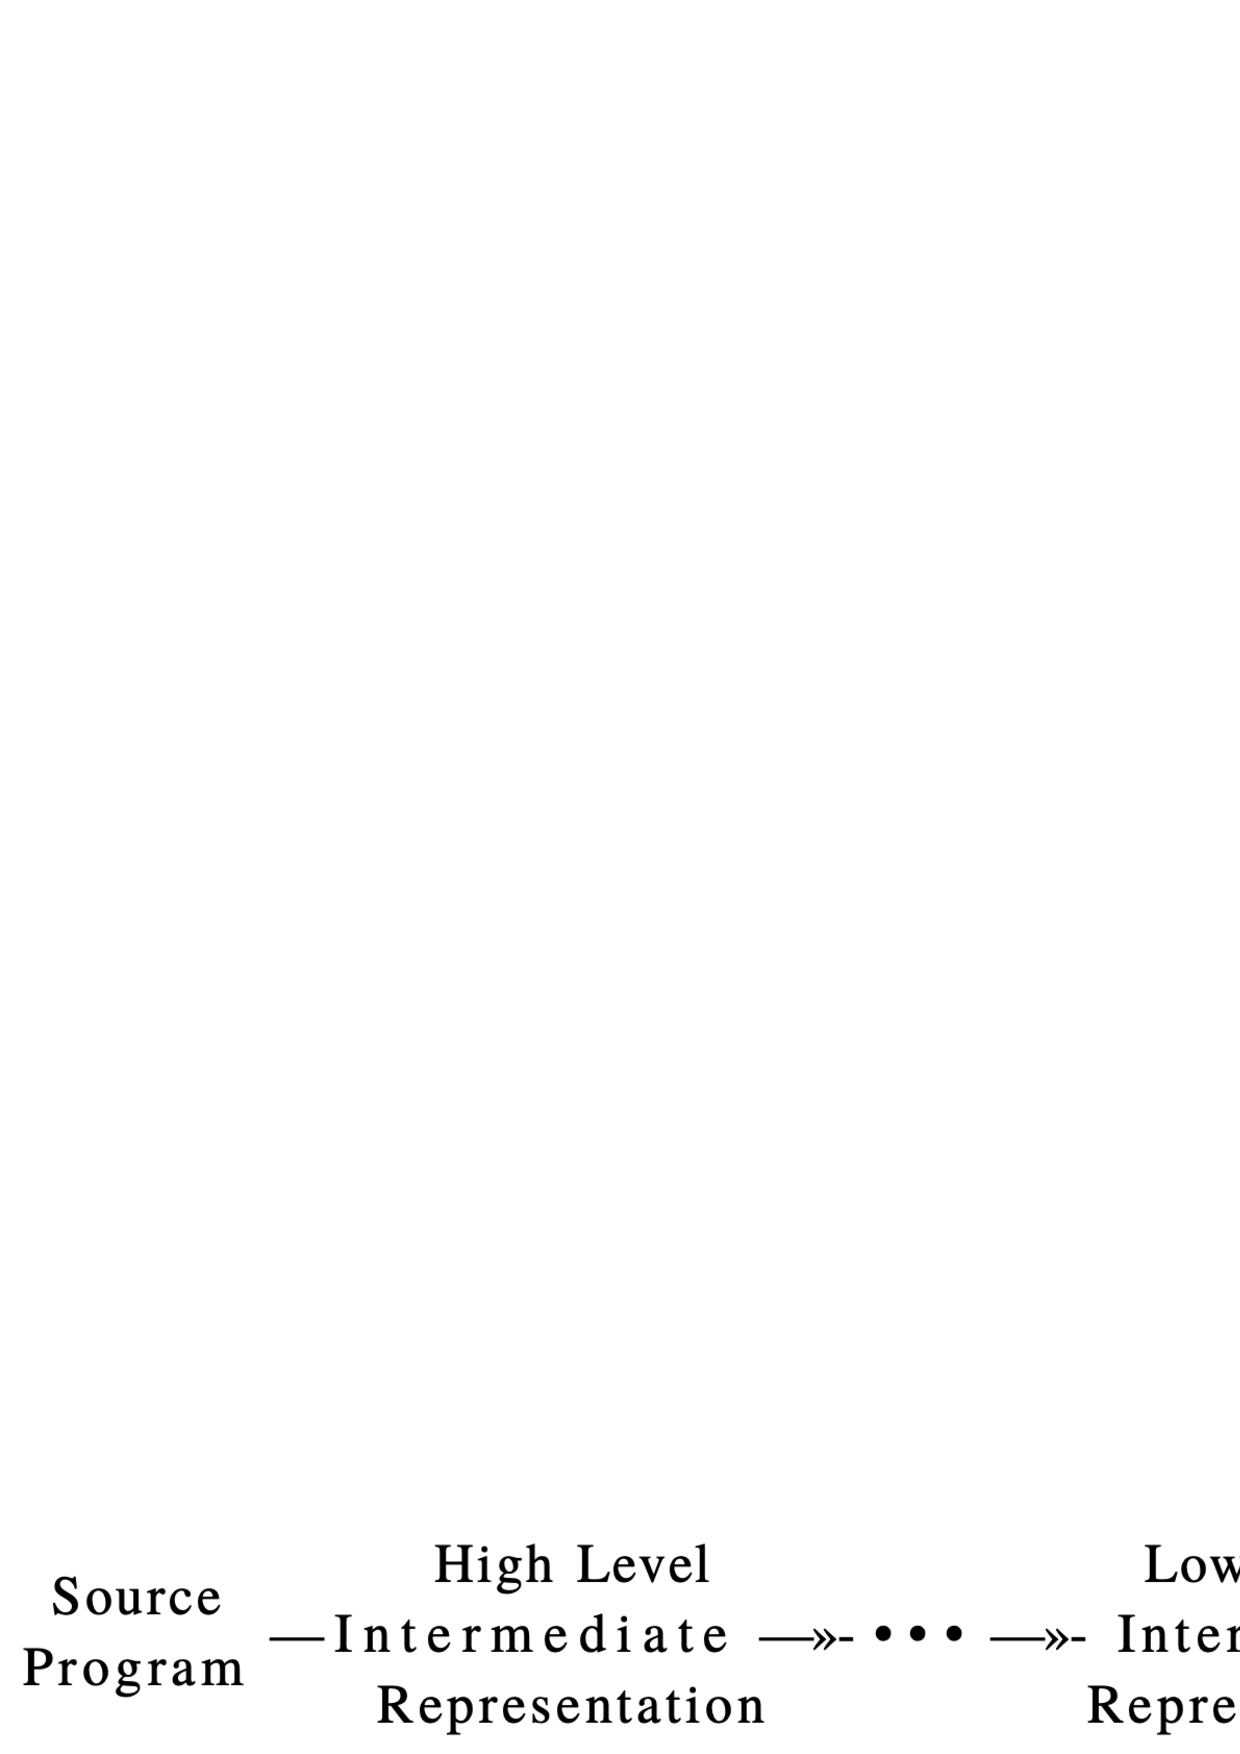
\includegraphics[width=\textwidth]{Imagens/abstraction-level-irs.pdf}
  \caption{Sequência de representações intermediárias}\label{fig:abstraction-level-irs}
  \small{Fonte:~\cite{aho2008compilers}}
\end{figure}
Uma das principais informações que deve ser preservada em uma IR é o fluxo de controle, isto é, a ordem em que as instruções do programa são executadas, como chamadas de função, \textit{loops} e condições.
Para garantir que o compilador mantenha a semântica correta do programa, o fluxo de controle deve ser repassado de alguma maneira durante o processo de tradução~\cite{cooper2014construindo}.
Uma das maneiras disso ser feito explicitamente é com o uso de continuações, que são funções que descrevem o próximo passo de uma computação em um ponto particular da execução do programa.

\subsection{CPS}\label{subsec:cps}

O estilo de passagem de continuações (CPS, do inglês \textit{continuation passing style}) é uma técnica de transformação de código que torna o fluxo de controle de um programa explícito, ao converter o estilo convencional de chamadas de função em chamadas que passam explicitamente o controle para a próxima etapa, conhecida como continuação (do inglês, \textit{continuation})~\cite{appel1992compiling}.
Em vez de retornar diretamente o resultado de uma função, o CPS transforma cada função para que, ao finalizar sua computação, ela invoque uma continuação que representa o próximo passo a ser executado no programa.
Assim, toda chamada de função se torna uma chamada de cauda.

Uma chamada de cauda (do inglês \textit{tail call}) ocorre quando a última instrução executada em uma função é uma chamada a outra função, sem que restem computações adicionais a serem feitas após essa chamada~\cite{muchnick1997advanced}.
Isso permite que a função atual libere seu quadro de ativação, otimizando o uso de memória, já que o compilador não precisa manter o estado da função anterior na pilha.
Em constraste, uma chamada que não é de cauda ocorre quando ainda restam operações após a chamada, como somas ou multiplicações, o que exige que o quadro de ativação da função atual permaneça na pilha até a conclusão dessas operações.

No Código~\ref{code:factorial_non_tail_call}, o exemplo da função fatorial demonstra uma chamada que não é de cauda, pois a chamada recursiva \texttt{factorial(n - 1)} não é a última operação a ser realizada.
A função precisa aguardar o retorno desta chamada para, então, multiplicar o resultado por \texttt{n}, o que impede a liberação do quadro de ativação até o término da multiplicação.

Em constrate, no Código~\ref{code:factorial_tail_call} como exemplo, tem-se uma versão da função fatorial que utiliza chamada de cauda.
A função auxiliar \texttt{go} acumula o valor do cálculo diretamente em seu argumento \texttt{a}, e a chamada recursiva \texttt{go (n - 1) (a * n)} é a última instrução a ser executada.
Como não há operações pendentes após a chamada recursiva, o compilador pode otimizar a função, reutilizando o espaço reservado para o quadro de ativação da função \texttt{go} para a chamada subsequente, tornando o cálculo mais eficiente.

\lstinputlisting[style=haskell, label=code:factorial_non_tail_call, caption={Função fatorial em Haskell}]{Code/factorial_non_tail_call.hs}

\lstinputlisting[style=haskell, label=code:factorial_tail_call, caption={Função fatorial em Haskell com chamada de cauda}]{Code/factorial_tail_call.hs}

O cálculo lambda, definido por~\citeonline{church1932set}, é um sistema formal que serve como base para a maioria das linguagens funcionais.
Ele é capaz de representar qualquer computação utilizando abstrações e aplicações através de reduções.
Sua sintaxe consiste em três regras simples que definem os elementos principais do sistema: variável, abstração e aplicação, conforme apresentados a seguir:

\begin{equation}\label{eq:lambda-calculus}
  e \Coloneqq x \mid \lambda x. e \mid e e
\end{equation}

A partir dessa sintaxe, um termo $e$ pode possuir apenas uma das três formas.
A primeira forma refere-se às variáveis, que representam identificadores no sistema.
A segunda forma, chamada de abstração, define uma função lambda: uma função que associa o identificador $x$ a um termo $e$, seu corpo, com $x$ vinculado ao termo $e$.
Finalmente, a aplicação ocorre quando um termo $e$ é aplicado a outro $e$, representando a chamada de uma função.

No cálculo lambda, as variáveis podem ser classificadas como livres ou ligadas, dependendo de seu contexto em um termo.
Variáveis são consideradas livres quando não estão associadas a uma abstração de função.
Por exemplo, no termo $\lambda x. y$, a variável $y$ é livre, pois não está ligada a nenhum parâmetro introduzido.
Em contraste, no termo $(\lambda x. x) y$, a variável $x$ está ligada dentro do corpo da abstração, enquanto $y$ permanece livre.
Um termo sem variáveis livres é denominado fechado ou combinador; por exemplo, $\lambda x. \lambda y. x y$ é um combinador, pois todas as variáveis estão ligadas às suas respectivas abstrações.

Para avaliar expressões no cálculo lambda, usamos três tipos de redução: $\alpha$, $\beta$ e $\eta$, que seguem as seguintes definições:

\begin{description}
  \item[$\alpha$-redução:] Renomeação de variáveis ligadas.
        \begin{align}
          \lambda x . e & \rightarrow \lambda y . e[y/x]\label{eq:alpha-reduction}
        \end{align}
        Note que, $e[y/x]$ indica a substituição de todas as ocorrências ligadas de $x$ por $y$ em $e$, desde que $y$ não ocorra livre em $e$. Por exemplo, $\lambda x. x + z \rightarrow_\alpha \lambda y. y + z$.

  \item[$\beta$-redução:] Aplicação de função.
        \begin{align}
          (\lambda x . e_1) e_2 & \rightarrow e_1 [e_2 / x]\label{eq:beta-reduction}
        \end{align}
        Aqui, $e_1[e_2/x]$ denota a substituição de todas as ocorrências ligadas de $x$ em $e_1$ por $e_2$. Para evitar conflitos com variáveis livres em $e_2$, aplica-se $\alpha$-redução prévia. Por exemplo, em $(\lambda x. \lambda y. x + y)(y + 1)$, renomeia-se $y$ para $z$ na abstração interna:
        \[
          (\lambda x. \lambda z. x + z)(y + 1) \rightarrow_\beta \lambda z. (y + 1) + z.
        \]

  \item[$\eta$-redução:] Expansão de função.
        \begin{align}
          \lambda x . (e \, x) & \rightarrow_\eta e \quad \text{se } x \notin \text{FV}(e)\label{eq:eta-reduction}
        \end{align}
        Tal que $\text{FV}(e)$ denota as variáveis livres em $e$. Por exemplo, $\lambda x. (\lambda y. y + 1) \, x \rightarrow_\eta \lambda y. y + 1$.
\end{description}

As reduções são responsáveis pela semântica operacional do cálculo lambda.
A $\alpha$-redução permite a renomeação de variáveis ligadas, enquanto a $\beta$-redução descreve a aplicação de funções, substituindo o parâmetro da função por um valor passado como argumento.
Por fim, a $\eta$-redução lida com a simplificação de funções quando elas aplicam diretamente seu argumento.

A transformação para CPS se baseia nessa estrutura formal.
No cálculo lambda tradicional, o fluxo de execução é implícito: as funções são aplicadas e seus resultados são retornados automaticamente.
No entanto, no CPS, o fluxo de controle é explicitamente representado como uma série de chamadas a funções.
Cada função, em vez de retornar diretamente um valor, recebe um argumento extra, a continuação, que indica o próximo passo da computação.

Por exemplo, a expressão $\lambda x. x + 1$ no cálculo lambda tradicional retornaria o valor $x + 1$. Ao transformar essa expressão para CPS, ela se torna $\lambda x. \lambda k. k (x + 1)$.

Aqui, $k$ é a continuação que processa o resultado $x + 1$.
Ao converter funções para CPS, o fluxo de controle do programa passa a ser gerenciado de forma explícita através de chamadas de função que encadeiam as etapas subsequentes.
Essa transformação traz diversas vantagens no contexto de compiladores, pois torna explícitas as informações normalmente implícitas na pilha de execução e, assim, abre espaço para a aplicação de uma série de otimizações~\cite{appel1992compiling}.  

Em primeiro lugar, o CPS expõe todas as chamadas de cauda, permitindo a eliminação de recursividade em cauda (TCO, do inglês \textit{tail-call optimization}).
Essa otimização possibilita que chamadas recursivas sejam realizadas sem o acúmulo de quadros de ativação na pilha, reduzindo o uso de memória e evitando estouros de pilha em programas fortemente recursivos.

Além disso, a natureza explícita das chamadas em CPS favorece a expansão \textit{inline} de funções.
Como cada chamada é clara e separada, o compilador pode substituir uma chamada de função por sua definição diretamente, reduzindo o \textit{overhead} de chamadas e potencialmente expondo outras oportunidades de otimização.

Outro ponto é a representação de \textit{closures}.
Uma \textit{closure} é uma estrutura que encapsula uma função junto a seu \textit{ambiente léxico} {---} o conjunto de variáveis livres capturadas do escopo externo no momento de sua criação.
Em CPS, como todo o contexto necessário à computação é passado de maneira explícita, o compilador consegue construir e manipular \textit{closures} com maior eficiência, uma vez que o ambiente da função está sempre disponível e bem definido.

A transformação para CPS também facilita a alocação de registradores.
Com o fluxo de controle explicitado, o compilador pode prever melhor o tempo de vida das variáveis e organizar os dados de forma que o uso de registradores seja maximizado e o número de acessos à memória minimizado~\cite{appel1992compiling}.

Por fim, como todo o fluxo de execução é expresso por chamadas encadeadas, o código gerado permite análises estáticas mais precisas.
O compilador pode, por exemplo, detectar com mais facilidade padrões de execução, dependências entre expressões e oportunidades de reordenação ou eliminação de código redundante.

Dessa forma, a conversão para CPS não apenas preserva a semântica da computação original, mas também fornece ao compilador uma estrutura rica e detalhada para aplicar otimizações de maneira eficaz.

O cálculo de continuações (do inglês, \textit{CPS-calculus}), conforme definido por~\citeonline{thielecke1997categorical}, é um sistema formal que leva o CPS além de seu uso tradicional como uma técnica de transformação de código, tratando-o como um modelo computacional por si só.
Enquanto o CPS é utilizado como uma IR em compiladores, o cálculo de continuações oferece uma estrutura para raciocinar formalmente sobre computações onde o fluxo de controle é explicitamente representado.
Os termos do cálculo de continuações, chamados de comandos, são descritos pelas seguintes regras:

\begin{equation*}
  M \Coloneqq x\langle \vec{x} \rangle \mid M\{x\langle \vec{x} \rangle = M\}
\end{equation*}

Vale ressaltar que \citeonline{appel1997shrinking} possuem uma sintaxe diferente para o cálculo de continuações, onde os termos são respectivamente representados como $k(\vec{x})$ e $\texttt{let }k(\vec{x}) = c \texttt{ in } b$.
Em razão da natureza prática e do público alvo deste trabalho, a notação adotada para o \textit{CPS-Calculus} será a do Appel.
Aqui, $k(\vec{x})$ representa um salto (do inglês \textit{jump}), isto é, uma chamada direta para a continuação $k$ com os parâmetros $\vec{x}$, essencialmente passando o controle para essa $k$.
Enquanto que $\texttt{let }k(\vec{y}) = c \texttt{ in } b$ representa um vínculo (do inglês \textit{binding}), onde a continuação $k$ com os parâmetros $\vec{y}$ é ligada dentro do comando $b$ com o corpo $c$.
Isto modela uma construção intermediária em que se define uma nova continuação que poderá ser chamada dentro de $b$ para prosseguir com a computação.

A tradução para CPS converte um código escrito em estilo direto (onde o controle de fluxo é implícito) para o estilo de passagem de continuações~\cite{flanagan1993essence}.
A principal ideia por trás dessa transformação é modificar as funções para que elas não retornem um valor diretamente, mas, em vez disso, passem o resultado para uma continuação.

\lstinputlisting[style=haskell, label=code:add, caption={Função soma em Haskell em Estilo Direto}]{Code/add.hs}

\lstinputlisting[style=haskell, label=code:add_cps, caption={Função soma em Haskell em CPS}]{Code/add_cps.hs}

Por exemplo, o Código~\ref{code:add} apresenta um programa na linguagem Haskell que soma dois números no estilo direto, retornando o valor após realizar o cálculo.
Já o Código~\ref{code:add_cps} mostra um programa equivalente em CPS\@.
Nesta versão, o controle de fluxo do programa é explícito, pois a função $k$ é chamada para processar o resultado da soma dos argumentos.

\lstinputlisting[style=haskell, label=code:factorial, caption={Função fatorial em Haskell em Estilo Direto}]{Code/factorial.hs}

\lstinputlisting[style=haskell, label=code:factorial_cps, caption={Função fatorial em Haskell em CPS}]{Code/factorial_cps.hs}

Para ilustrar melhor, o Código~\ref{code:factorial} apresenta um programa em Haskell que calcula o fatorial no estilo direto, utilizando funções definidas para multiplicação e subtração.
No Código~\ref{code:factorial_cps}, um programa similar em CPS é definido, com as funções auxiliares também transformadas para CPS\@.
Na função \texttt{factorialCps} é possível notar duas funções lambda (continuações anônimas): a primeira com parâmetro \texttt{nMinus1} e a segunda com parâmetro \texttt{factNMinus1}.
A primeira continuação guarda o resultado da operação $n - 1$, enquanto a segunda recebe recursivamente o cálculo do fatorial de $n - 1$, multiplica por $n$ e finalmente passa o resultado para a continuação $k$.
Note que aqui, quando \texttt{subCps} retorna, seu resultado é vinculado a \texttt{nMinus1}; quando \texttt{factorialCps} retorna, seu resultado é vinculado a \texttt{factNMinus1}.
As variáveis $n$ e $k$ são capturadas do contexto externo pelas \textit{closures}, mantendo seu valor original.

Outro fato importante a ser observado nos códigos apresentados é a tipagem das funções.
Na função de soma, definida no Código~\ref{code:add}, a função tem tipo $Int \rightarrow Int \rightarrow Int$, ou seja, ela recebe dois inteiros e retorna um inteiro.
Já a função de soma em CPS, definida no Código~\ref{code:add_cps}, possui o tipo $Int \rightarrow Int \rightarrow (Int \rightarrow r) \rightarrow r$. Isso significa que a função recebe dois inteiros e uma continuação, que é uma função de tipo $Int \rightarrow r$, onde \texttt{r} pode ser qualquer tipo, e retorna esse mesmo tipo \texttt{r}.

Essa transformação de tipo reflete a diferença fundamental entre o estilo direto e o CPS\@: em vez de retornar um valor diretamente, a função em CPS recebe uma continuação que especifica o próximo passo da computação.
O mesmo padrão pode ser observado nas funções para o cálculo do fatorial nos Códigos~\ref{code:factorial} e~\ref{code:factorial_cps}.
No estilo direto, a função \texttt{factorial} tem o tipo $Int \rightarrow Int$, enquanto na versão CPS, a função \texttt{factorialCps} tem o tipo $Int \rightarrow (Int \rightarrow r) \rightarrow r$.

Essa correspondência entre os tipos não é uma coincidência.
Como discutido por~\citeonline{torrens2019calculo}, uma função em estilo direto com tipo $A \rightarrow B$ pode ser transformada em uma função em CPS com o tipo $A \rightarrow (B \rightarrow \perp) \rightarrow \perp$.
Aqui, $\perp$ representa o tipo dos valores que nunca retornam, uma característica associada ao estilo de passagem de continuações, onde as funções são compostas de forma a encadear continuações até que a execução termine de maneira explícita.

Este exemplo simples da função fatorial em CPS ilustra as dificuldades inerentes ao uso de continuações explícitas, como a verbosidade do código e a complexidade de compreensão, mas não sua inadequação para compilação.
Apesar desses desafios, o CPS se mostra extremamente adequado para a aplicação de otimizações, sendo uma escolha eficiente para representações intermediárias, especialmente em cenários onde o desempenho é essencial.


\begin{frame}{Teoria de Tipos}
    % \begin{itemize}
    %     \item \citeonline{appel1998ssa} demonstra a equivalência entre código funcional e uma representação na forma SSA

    %     \item []

    %     \item [] \begin{figure}
    %         \centering
    %         \includegraphics[width=.8\textwidth]{Figuras/ssa-funcional.png}
    %         \caption{Representações Equivalentes \cite{appel1998ssa}}
    %         \label{fig:conv1}
    %     \end{figure}
    % \end{itemize}
\end{frame}

% \chapter{Sistema Damas Milner}\label{ch:damas-milner}

% O sistema Damas-Milner é um sistema de tipos para o cálculo lamda, com polimorfismo paramétrico criado por Hindley, Damas e Milner para a linguagem de programação de propósito geral ML \cite{HINDLEY1969, MILNER1978, DAMAS1984}.
% Conforme destacado por \citeonline{DAMAS1982}, a linguagem ML possuia fortes aspectos como flexibilidade (através do polimorfismo), robustez (devido à \textit{soundness} semântica) e fortes mecanismos de detecção de erros em tempo de compilação.
% Este equilíbrio, permite que linguagens funcionais como Haskell e OCaml herdem suas características e usem este sistema como base em seus sistemas de tipos.

% \section{Algoritmo W}\label{sec:w-algo}

\chapter{Sistema Damas-Milner}\label{ch:damas-milner}

O sistema Damas-Milner, introduzido por Robin Milner e posteriormente formalizado em maior detalhe por Luis Damas \cite{MILNER1978, DAMAS1982}, é um dos sistemas de tipos mais influentes para linguagens funcionais.
Este sistema tem como principal característica a inferência automática de tipos polimórficos, sem a necessidade de anotações explícitas por parte do programador, como ocorre em linguagens como ML, Haskell e OCaml.
A sua base é o cálculo lambda com polimorfismo paramétrico, permitindo que funções possam operar sobre múltiplos tipos de maneira genérica.

A introdução do sistema Damas-Milner trouxe duas contribuições principais: a definição de um sistema de tipos que é robusto, garantindo propriedades como \textit{soundness} (consistência semântica), e a criação de um algoritmo, o Algoritmo W, capaz de inferir o tipo mais geral (também chamado de \textit{principal type-scheme}), conforme demonstrado em \citeonline{DAMAS1984}.
Como resultado, a linguagem ML e suas derivadas se tornaram notórias por fornecer ao programador a capacidade de escrever programas sem erros de tipo detectáveis durante a compilação, permitindo um desenvolvimento mais seguro e robusto \cite{MILNER1978, DAMAS1984}.

A sintaxe do sistema DM define as expressões e os tipos usados no processo de inferência.
Abaixo, segue a gramática das expressões e tipos:

\begin{equation}\label{eq:dm-syntax}
  \begin{array}{ll}
    \text{Variáveis}         & x                                                                                 \\
    \text{Expressões}        & e ::= x \mid e \ e' \mid \lambda x.e \mid \texttt{let} \ x = e \ \texttt{in} \ e' \\
    \\
    \text{Variáveis de tipo} & \alpha                                                                            \\
    \text{Tipos primitivos}  & \iota                                                                             \\
    \text{Tipos}             & \tau ::= \alpha \mid \iota \mid \tau \rightarrow \tau
    \alpha                                                                                                       \\
    \text{Schemes}           & \sigma ::= \forall \alpha. \sigma \mid \tau                                       \\
  \end{array}
\end{equation}

Na sintaxe, $x$ representa variáveis que podem ser nomes de qualquer identificador, e $e$ descreve expressões que podem ser variáveis, aplicações de função, funções anônimas ou declarações \texttt{let}, que introduzem polimorfismo através de generalização de tipos.
As variáveis de tipo $\alpha$ são usadas para representar tipos genéricos.
Os tipos primitivos $\iota$ são usados para representar tipos constantes.
Tipos $\tau$ podem ser tanto variáveis de tipo quanto funções entre tipos.
Por fim, $\sigma$ denota \textit{schemes}, ou tipos polimórficos, que podem quantificar variáveis de tipo, permitindo reutilização de tipos genéricos em diferentes contextos.

O polimorfismo no sistema Damas-Milner é introduzido pelas expressões \texttt{let}, que permitem a generalização de tipos. Ao declarar uma variável ou função usando \texttt{let}, o tipo inferido é generalizado para ser reutilizado em diferentes contextos. Isso significa que, ao declarar uma função como $\texttt{id} = \lambda x.x$, o sistema deduz o tipo mais geral $\forall \alpha. \alpha \rightarrow \alpha$, que pode ser usado com diferentes tipos conforme necessário.

A inferência de tipos envolve dois processos principais: generalização e instanciação.
A generalização ocorre quando o sistema identifica que uma expressão pode ser tipada com um tipo mais geral, permitindo que seja reutilizada de maneira polimórfica.
Já a instanciação ocorre quando um tipo polimórfico é aplicado a um tipo concreto, especializando-o para um uso específico.
Esse mecanismo garante a flexibilidade do sistema, ao mesmo tempo que mantém a segurança garantida pela inferência de tipos.

Por exemplo, considere a expressão $\texttt{let id} \ = \lambda x.x \ \texttt{in} \ (\texttt{id} \ \texttt{1}, \ \texttt{id} \ \texttt{`a'})$.
O sistema generaliza o tipo de $\texttt{id}$ para $\forall \alpha. \alpha \rightarrow \alpha$, e instancia este tipo tanto para inteiros quanto para caracteres nas duas aplicações subsequentes.

% Substituições

% Variáveis livres

% Regras de inferência

\section{Algoritmo W}\label{sec:w-algo}

% Algoritmo de unificação

% Algoritmo W

\section{Formalização}\label{sec:formalizacao}
\section{Implementação}\label{sec:implementacao}

Partindo para a parte prática do trabalho, os módulos e funções serão apresentados de maneira gradual, de modo a facilitar o entendimento do fluxo inteiro do programa.
Vale destacar aqui que é feito também a implementação do sistema Hindley-Milner, porém, como este foi feito somente para poder usar o sistema de continuações de maneira mais cômoda, não será entrado em detalhes nos que dizem respeito à esse sistema de tipos.
Inicialmente, na Subseção~\ref{subsec:cps-adt}, será discutido sobre a maneira como foi representado o sistema de tipos.
Em sequência, a Subseção~\ref{subsec:cps-translations} trará detalhes sobre a implementação das funções de tradução de cálculo lambda simplesmente tipado para CPS.
Posteriormente, a Subseção~\ref{subsec:cps-inferer} irá tratar da inferência em si, juntamente da verificação do tipo.
Por fim, a geração de código abordada na Subseção~\ref{subsec:cps-code-gen} serve como uma maneira de se testar a tradução do código.

\subsection{Tipos de Dados}\label{subsec:cps-adt}

Para representar os comandos, bem como os tipos do sistema, foram utilizados tipos de dados algébricos (ADTs, do inglês \textit{algebraic data types}), disponíveis no Listing~\ref{code:cps-adt}.

\lstinputlisting[style=haskell, label=code:cps-adt, caption={Definição dos tipos de dados}]{Code/Type-Inferer/CPSTyping.hs}
Para os comandos, dois construtores podem ser observados, o \texttt{Jump} e o \texttt{Bind}, sendo responsáveis por construir respectivamente os comandos de \textit{Jump}, onde há um salto \texttt{Id} com \texttt{[Id]} parâmetros.
Sendo assim, o salto $k(x)$ seria representado por este ADT: $\mathtt{Jump\ k\ [x]}$.
E o comando \textit{Bind}, onde há outro \texttt{Command} definido recursivamente, a função \texttt{Id} com argumentos \texttt{[Id]} e por fim outro \texttt{Command} também definido recursivamente.
O \textit{bind} $\mathtt{let}\ k(x) = k(x)\ \mathtt{in}\ k(x)$, portanto seria definido pelo seguinte ADT: $\mathtt{Bind\ (Jump\ k\ [x])\ k\ [x]\ (Jump\ k\ [x])}$.

Os tipos, foram representados com dois tipos algébricos diferentes, um para os monotipos $\mathtt{CPSMonoType}$, e uma para os politipos $\mathtt{CPSPolyType}$.
As variáveis do monotipo são construídas a partir dos construtores $\mathtt{TVar\ Id}$ e $\mathtt{TInt}$, onde no primeiro, o $\mathtt{Id}$ serve para obter a variável de tipo atribuída àquela variável, enquanto que as funções que não retornam são representadas as partir do construtor de negação $\mathtt{TNeg\ [CPSMonoType]}$ sendo os argumentos dela definidos recursivamente sobre si.
O contexto por sua vez, é um tipo que utiliza o $\mathtt{Data.Map}$ disponível no pacote \textit{containers} para mapear uma variável para um tipo polimórfico.
As substituições são representadas utilizando o mesmo $\mathtt{Data.Map}$, onde desta vez é mapeado uma variável de tipo para um monotipo.

\subsection{Traduções}\label{subsec:cps-translations}
Para facilitar os testes efetuados e ainda tornar o fluxo de execução mais direto, foram implementas as funções de tradução de expressões e de tipos de acordo com as definições das Seções~\ref{subsec:cps-translation} e~\ref{subsec:typed-cps-translation}.

\lstinputlisting[style=haskell, label=cps:cbn-initial-cont, caption={Continuação inicial}]{Code/Type-Inferer/CPS_initial_cont.hs}
Para todas as computações, um contexto inicial precisa conter a continuação inicial.
Este será o objeto a ter seu tipo inferido.
Afim de praticidade, esta continuação será sempre a mesma, dada por `k', como mostrado no Código~\ref{cps:cbn-initial-cont}.

\lstinputlisting[style=haskell, label=cps:cbn-expr-translation, caption={Tradução das expressões para CBN}]{Code/Type-Inferer/CPS_CBN_expr_translation.hs}
No Código~\ref{cps:cbn-expr-translation}, são apresentadas as funções responsáveis para traduzir as expressões para CBN.
O ponto de partida desta computação será a função $\mathtt{cbnExprTrans \dblcolon Expr \to Command}$, onde ela irá receber a expressão em cálculo-$\lambda$ e retornará o comando traduzido.
Sua responsabilidade é criar as mônadas de estado que farão o controle do índice das variáveis frescas necessárias e chamar as funções de tradução passando a continuação inicial.

Tomando como exemplo a função identidade em cálculo-$\lambda$ ($\lambda x.\ x$), é possível perceber como os termos crescem em CPS.
Isto torna o desenvolvimento diretamente neste cálculo não apropriado, mas ainda, nota-se que a implementação da função de tradução é bastante direta em relação a sua definição formal.
Os únicos pontos de atenção são em relação à geração das variáveis frescas, mas que como foi dito anteriormente, não eram completamente necessários, visto que eles são ligados imediatamente.
Ao traduzir então a função, tem-se que o equivalente em CPS é o mostrado no Código~\ref{cps:id-cps-cbn}.
\lstinputlisting[style=haskell, label=cps:id-cps-cbn, caption={Tradução da função identidade em CBN}]{Code/Type-Inferer/CPS/id-cbn.cps}
Este comportamento fica ainda mais visível quando uma função um pouco maior é traduzida, por exemplo o numeral de Church dois ($\lambda f.\ \lambda x.\ f\ (f\ x)$).
Sua tradução portanto é mostrada no Código~\ref{cps:church-two-cps-cbn}.
\lstinputlisting[style=haskell, label=cps:church-two-cps-cbn, caption={Tradução do numeral de Church ``2'' em CBN}]{Code/Type-Inferer/CPS/church-two-cbn.cps}
De maneira semelhante, foram feitas as mesmas funções utilizadas no \textit{call-by-name}, porém adaptadas para o CBV, respeitando as diferenças presentes na definicão formal da função.
\lstinputlisting[style=haskell, label=cps:cbv-expr-translation, caption={Tradução das expressões para CBV}]{Code/Type-Inferer/CPS_CBV_expr_translation.hs}
A partir dessas diferenças nas definições, nota-se também particularidades nas traduções destas, por exemplo ao traduzir a mesma função identidade, em CBV, é obtido o resultado apresentado no Código~\ref{cps:id-cps-cbv}.
\lstinputlisting[style=haskell, label=cps:id-cps-cbv, caption={Tradução da função identidade em CBV}]{Code/Type-Inferer/CPS/id-cbv.cps}
Neste exemplo da função identidade, pouca diferença entre as duas estratégias de avaliação pode ser notada.
Isso se deve não ao tamanho da expressão, e sim dos elementos desta.
Neste caso, há somente uma abstração lambda com uma variável.
A seguir, é exibido novamente o numeral de Church dois, porém para o CBV, onde mais diferenças podem ser observadas.
O motivo disto é os elementos da função, que diferentemente da identidade, conta com mais construtores para representá-la, exibido no Código~\ref{cps:church-two-cps-cbv}.
\lstinputlisting[style=haskell, label=cps:church-two-cps-cbv, caption={Tradução do numeral de Church ``2'' em CBV}]{Code/Type-Inferer/CPS/church-two-cbv.cps}

Mostrado anteriormente no Código~\ref{cps:id-cps-cbn}, a expressão CPS resultante da tradução da função identidade em CBN difere da mesma traduzida em CBV, presente no Código~\ref{cps:id-cps-cbv}.
O mesmo pode ser observado ao traduzir a função identidade tipada.
Por exemplo, ao executar a função para a identidade em CBN, o tipo obtido é $\neg\neg(\neg\neg\alpha,\ \neg\alpha)$.
Já em CBV, para a mesma função, tem-se que o tipo traduzido é $(\alpha,\ \neg\alpha)$.

Para raciocinar sobre os tipos do sistema, tem que ser levado em consideração o que estes representam, contradições.
Ao tomar como exemplo o tipo resultante da função identidade em CPS a partir da tradução por valor (CBV), isto é, $(\alpha,\ \neg\alpha)$\footnote{Apesar de estar sendo traduzido o tipo da função identidade, como esta tradução é feita para os tipos simples, note que aqui, está sendo representado monomorficamente pois não há a generalização do $\alpha$.}, deve-se pensar que este representa o absurdo de ter $\alpha$ como argumento e $\neg\alpha$ como continuação, ao mesmo tempo.

\lstinputlisting[style=haskell, label=cps:cbn-type-translation, caption={Tradução dos tipos para CBN}]{Code/Type-Inferer/CPS_CBN_type_translation.hs}
Aqui no Código~\ref{cps:cbn-type-translation}, a função responsável por traduzir um tipo utilizando a estratégia \textit{call-by-name}, a função $\mathtt{cbvTypeTranslation \dblcolon LambdaMonoType \to CPSPolyType}$ irá receber um tipo simples no cálculo-$\lambda$ simplesmente tipado, e retornar um tipo polimórfico em CPS.
Perceba que na definição, o retorno era um tipo simples em CPS. 
Essa diferença é justificada ao se observar o corpo desta função, onde há a definição da função $\mathtt{cbvTrans}$.
Esta é quem efetivamente faz a computação, pois é nela que acontece o casamento de padrões para determinar o tipo sendo traduzido.
Ainda, esta função retorna um tipo polimórfico pelo fato de que em momento posterior a essa tradução, a subtipagem do tipo traduzido e do tipo inferido precisa ser verificada.

\lstinputlisting[style=haskell, label=cps:cbv-type-translation, caption={Tradução dos tipos para CBV}]{Code/Type-Inferer/CPS_CBV_type_translation.hs}
Para que essas duas funções de tradução de tipos (CBN e CBV) sejam usadas do mesmo modo, elas seguem a messma assinatura. 
Seus comportamentos são o mesmo, a diferir somente nas diferenças das definições da função, isto é, como é feita a tradução.

O sistema de tipos proposto neste trabalho, entretanto, é polimórfico, ou seja, aqui há a adição de variáveis de tipos quantificadas.
Sendo assim, esta função de tradução, se aplicando neste caso de uso, não necessariamente retornará o tipo mais geral de uma expressão, mas sempre um subtipo deste.

\subsection{Inferência}\label{subsec:cps-inferer}
% Explicar inferência
% \lstinputlisting[style=haskell, label=cps:typing, caption={Definição dos tipos de dados}]{Code/Type-Inferer/CPSTyping.hs}
% Explicar código

\subsection{Geração de Código}\label{subsec:cps-code-gen}
Uma vez que as provas de completude e consistência não estavam no escopo deste trabalho e a validação do algoritmo se deu por meio de testes, um conjunto considerável de testes foi construído.
Para isolar os testes, ou seja, testar as funções de maneira independente para garantir que, se a inferência apresentasse algum erro, fosse certo que o erro estaria na inferência e não por conta de uma tradução incorreta, dois teoremas apresentados em~\cite{plotkin1975call} foram utilizados.

Este teorema, chamado de Teorema da Simulação, válido tanto para \textit{call-by-name} quanto para \textit{call-by-value}, afirma que, dado um programa $M$ em cálculo-$\lambda$, o resultado de sua computação há de ser o mesmo que o resultado da computação da tradução para CPS com a função identidade.
Ou seja, simulando a execução do programa feito em cálculo-$\lambda$ no cálculo de continuações.
Ou então, formalmente, $Eval(M) = Eval([M] (\lambda x.\ x))$, onde a função $Eval$ é responsável por avaliar uma expressão, efetivamente a computando.

Foi implementada a simulação do cálculo-$\lambda$ no cálculo de continuações a partir das funções de tradução para programas que computam os numerais de Church.
Isto é feito computando a função $\lambda$ onde, é incrementado o valor que representa o número de aplicações feitas (essencialmente como um numeral de Church é computado), passando como continuação a função identidade.
Fazendo com que assim, a função lambda que representa um numeral de church é simulada pelo cálculo de continuações.

\lstinputlisting[style=haskell, label=cps:code-gen, caption={Geração de código para computação de numerais de Church}]{Code/Type-Inferer/CPS_code_gen.hs}
O código Haskell gerado pode ser dividido em três partes principais, o cabeçalho de caráter informativo, que explicita o programa em cálculo-$\lambda$ de entrada para ter gerado aquele programa em CPS.
Em seguida, há a definição das funções $\mathtt{cbn}$ e $\mathtt{cbv}$, ou seja, os programas correspondente em CPS para as duas traduções daquela entrada.
Por fim, a última parte é responsável pela computação do numeral de Church, as funções definidas irão calcular o número representado pelas expressões em CPS e retornar por fim uma tupla contendo o resultado do calculado pelo \textit{call-by-name} e \textit{call-by-value} respectivamente.

Ao se traduzir o numeral de Church 0 representado em cálculo-$\lambda$ por $\lambda f.\lambda x.\ x$, para CBN e CBV, tem-se:
\lstinputlisting[style=haskell, label=cps:church-zero-cps-cbn, caption={Tradução do numeral de Church ``0'' em CBN}]{Code/Type-Inferer/CPS/church-zero-cbn.cps}
\lstinputlisting[style=haskell, label=cps:church-zero-cps-cbv, caption={Tradução do numeral de Church ``0'' em CBV}]{Code/Type-Inferer/CPS/church-zero-cbv.cps}
Desta forma, o código gerado ao se traduzir esta função, é ilustrado a seguir:
\lstinputlisting[style=haskell, label=cps:church-zero-output, caption={Código gerado ao traduzir o numeral de Church ``0''}]{Code/Type-Inferer/CPS/church-zero.hs}
Ao executar o código e chamar a função $\mathtt{main}$ deste programa, o resultado obtido é justamente a computação do numeral para as duas traduções, ou seja, $\mathtt{(0,\ 0)}$.

\subsection{Fluxo Principal}\label{subsec:cps-main-program}
O fluxo completo de execução do programa principal contempla todas as funções apresentadas nesta seção, com a adição de funções auxiliares.
Essas são aplicadas em sequência, de modo a realizar uma série de ações.

Inicialmente, é passado o caminho de um arquivo contendo um programa em cálculo-$\lambda$ com adição do `let'.
O conteúdo então é processado pelo \textit{parser} e representado pelos tipos de dados algébricos para o cálculo lambda.
Uma vez que o programa já está sendo representado pelos ADTs, e ainda tem seu tipo inferido, é possível iniciar o processamento descrito pelas funções apresentadas.
A primeira delas é a tradução para CPS tanto em \textit{call-by-name} quanto em \textit{call-by-value}, as exibindo logo em seguida.
Com as traduções da expressão feitas o código Haskell já pode ser gerado, salvando assim no diretório \texttt{output} com mesmo nome do arquivo de entrada.
Como passo posterior, tem-se a tradução dos tipos para ambas as estratégias de avaliação.
Os passos finais envolvem a inferência de ambas as traduções, juntamente da verificação de subtipagem, onde esta informará se o tipo traduzido é um subtipo do inferido.

\lstset{extendedchars=false, escapeinside=''}
\lstinputlisting[style=output, label=cps:main-execution, caption={Execução do programa principal}]{Code/Type-Inferer/CPS_main_execution.cps}
Ao executar o programa com o comando \texttt{cabal run}, passando também o arquivo de entrada \texttt{input/church-zero.in}, é processado e exibida todas as informações que foi citada anteriormente, inclusive a geração do código Haskell em \texttt{output/church-zero.hs}.
É possível perceber que na saída do programa, é mostrado o tipo traduzido (na sequência da mensagem ``\textit{Expected Continuation Type:}'') e o tipo inferido (que sucede a mensagem ``\textit{Inferred Continuation Type:}'').
Logo em seguida, o questionamento ``\textit{Do the types match?}'' é o trecho da saída que compete à subtipagem, retornando ``\textit{Yes}'' caso esse seja um subtipo deste, o que indica uma inferência compatível com a tradução ou ``\textit{No}'' caso a verificação falhe, indicando uma inferência incorreta.

\lstset{extendedchars=false, escapeinside=''}
\lstinputlisting[style=output, label=cps:execution-generated, caption={Execução do programa gerado}]{Code/Type-Inferer/CPS_execution_generated.cps}
Ainda, a compilação e execução do código Haskell gerado pode ser conferida no Código~\ref{cps:execution-generated} acima, ilustrando exatamente o comportamento detalhado anteriormente.


\section{Conclusão}\label{sec:conclusao}
As IRs são muito importantes na compilação, elas permitem otimizar muitos processos para assim tornar mais eficiente o código.
Os sistemas de tipos permitem provas de propriedades de um sistema, garantindo que programas tenham comportamento esperado.
Por exemplo, uma função que opera sobre um conjunto numérico, utilizando um sistema de tipos, seria possível identificar um uso incorreto desta função ao passar um argumento de outro tipo, podendo assim impedir que a função compute para evitar um comportamento inesperado.
Sendo assim, pode-se dizer que o sistema de tipos adiciona uma camada de segurança ao programa.

Uma das maiores motivações de adicionar essa camada de segurança na representação intermediária, ou seja de desenvolver um sistema de tipos para o CPS, é extender a prova de programas para as etapas seguintes em que o sistema já não tem mais ciência dos tipos, ou seja, o ligador (do inglês \textit{linker}).
Considerando o cenário onde um programa possua milhares de arquivos fonte, com IRs não tipadas, as provas das propriedades de funções definidas em um arquivo somente são passadas para outra caso estes sejam compilados juntos -- o que se torna inviável em programas tão grandes.
Já com uma IR tipada, se uma função $f$ definida em um arquivo espera receber um inteiro for utilizada em outro módulo onde na verdade está sendo passado como argumento uma cadeia de caracteres, o erro seria facilmente identificado no momento da ligação (do inglês \textit{linking}), não havendo a necessidade de recompilar o arquivo que contém a função ou ainda todos os que o utilizam.

Mesmo que o sistema não funcione para o `let' no CBV, a tradução está correta, onde isso significa respeitar o teorema da simulação.
Isto é, no caso de uma implementação não tipada da tradução, não haveria problemas em simular a expressão lambda no cálculo de continuações.
Como a tradução para CBV não preserva tipos, um dos trabalhos futuros incluiria a correção deste.
Para tal, seria necessário propor um outro sistema de tipos polimórfico para o cálculo de continuações onde, sejam distinguidos tipos e cotipos dentre os argumentos para que o algoritmo de inferência saiba quando utilizar um ou outro.

Outro trabalho futuro são as provas de consistência e completude do sistema de tipos proposto em relação ao algoritmo de inferência.
Neste trabalho foram executados alguns casos de testes que demostraram empiricamente que o algoritmo está correto.
Em conjunto, um avanço seria a criação de um compilador que faça uso desta IR tipada, colocando em prática toda a teoria aqui apresentada.


% ----------------------- %
% ELEMENTOS PÓS-TEXTUAIS
% ----------------------- %
\postextual

% Referências bibliográficas
\bibliography{referencias}										% Elemento Obrigatório

%\include{PosTextuais/Glossario}							% Elemento Opcional
%\include{PosTextuais/Apendices}							% Elemento Opcional
%\include{PosTextuais/Anexos}									% Elemento Opcional
%\include{PosTextuais/IndiceRemissivo}				% Elemento Opcional

\end{document}

% ----------------- %
% Fim do Documento
% ----------------- %
